\section{Data preparation}

Caching is intended to help with file retrieval from a distant server. A sequence of requests is called a request trace. Each entry to the request trace contains the time of the request, file ID, and optionally some metadata (size, type, etc.). To develop and test the algorithm the required data is split into two cases - the case of real-world data and the case of synthetic data. Real-world data is suitable for final algorithm evaluation since it represents real end-user request pattern. However, during the development process, it is better to use synthetic data, since it provides a controlled environment with a fixed number of unique items in which the behavior of the system is easier to understand.

\subsection{Synthetic data}

The primary challenge in the task of creation of the synthetic traces is to create them in such a way that they represent close to real-world data. A number of studies have been conducted to show that the popularity of files requested from web servers is distributed by Zipf's law\cite{10}. At the same time, the arrival time of the requests can be modeled as a Poisson process\cite{11}. This two facts will form the basis of synthetic trace generation.

While relying on previously described facts, we will be able to create synthetic traces, in the real world the popularity of the objects is not static with the passage of time since new content appears all the time and old content becomes less popular. That is why we have decided to represent synthetic traces in two cases. The first case is the case with the static popularity. The second case is the case with nonstatic popularity. In this case, the population is splitted in two equal sized parts. The first half of the population, as in the case one, has static Zipf distributed popularity. The popularity of the second half of the population is also distributed by Zipf's law but the popularity is randomly shuffled every predefined time frame $ t_0 $.

\subsection{Real-world data}

\begin{figure}[b!]
	\centering
	
	\begin{subfigure}[b]{0.49\linewidth}
		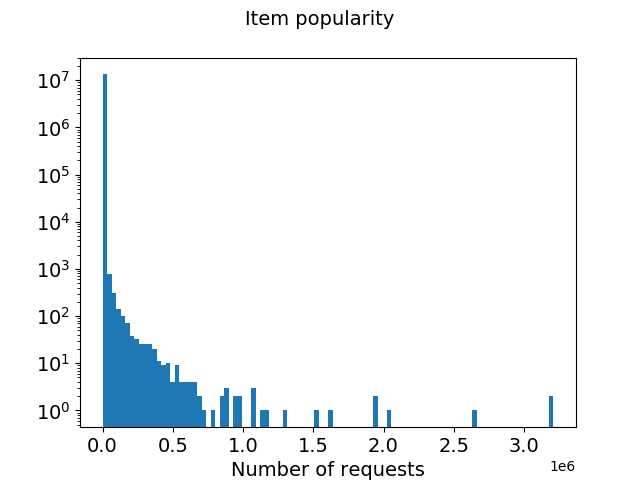
\includegraphics[width=\linewidth]{pics/real_item_pop.png}
		\caption{5 day trace.}
	\end{subfigure}
	\begin{subfigure}[b]{0.49\linewidth}
		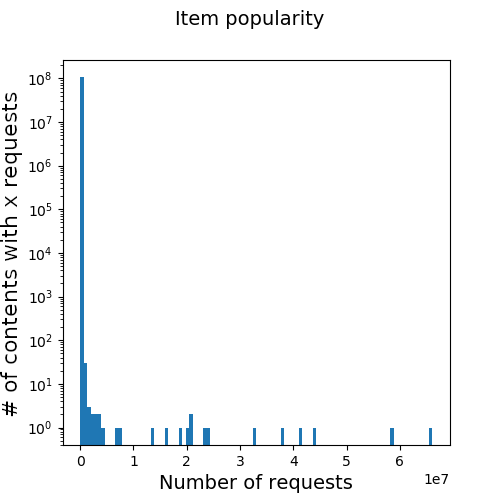
\includegraphics[width=\linewidth]{pics/real2_item_pop.png}
		\caption{30 day trace.}
	\end{subfigure}
	\caption{Trace item popularity.}
	\label{fig:pop_1}
\end{figure}

\begin{table}[h!]
	\centering
	\begin{tabular}{| c | c | c |}
		\hline
		& 5-day trace & 30-day trace \\
		\hline 
		Total requests & $ 417 * 10^6 $ & $ 2.22 * 10^9 $ \\ 
		Time span & 5 days & 30 days \\
		Unique items & $ 13.27 * 10^6 $ & $ 113.15 * 10^6 $ \\
		Request rate & 966.97 requests/s & 856.48 requests/s \\
		Min object size & 3400 bytes & 1 bytes \\
		Max object size & 1.15 gigabytes & 10.73 gigabytes \\ 
		Mean object size & $ 4.85 * 10^5 $ bytes & $ 3.63 * 10^5 $ bytes \\
		\hline
	\end{tabular}
	\caption{Akamai request traces information.}
	\label{table:1}
\end{table}

The real world data has been obtained from Akamai content delivery network\cite{12}. We were able to get access to two request traces collected from two different vantage points of the Akamai network. The first one spans over 5 days and further will be referred to as the 5-day trace. By analogy, the second one spans over 30 days and will be referred to as the 30-day trace. The detailed information about the traces you can find in the Table \ref{table:1} below.



As you can see in the Table \ref{table:1}, request traces contain not only the ID and the time of request arrival but also the size of the object. For now, we will consider that the size of all of the objects is equal and caching one object consumes one discreet place in the cache. The size of the object may later prove itself useful as a metadata feature for the neural network to process. This request traces are going to be used to evaluate the performance of the proposed algorithm and to compare it with other reviewed approaches.

Figure \ref{fig:pop_1} shows the distribution of popularity of objects in the traces. A large number of the objects are requested only once (notice the logarithmic scale of the y axis of the figure). Pure LRU policy is always putting such objects in the cache potentially removing a more popular object from the cache. Such behavior leads to a reduced cache hit ratio and should be avoided by the proposed caching policy.